\documentclass[a4paper,12pt]{jarticle}
\newcommand{\vect}[1]{\mbox{\boldmath${#1}$}}
\setlength{\textwidth}{170mm}       % テキストの幅
\setlength{\textheight}{260mm}      % テキストの高さ
\setlength{\oddsidemargin}{-5mm}    % 偶数ページの左マージン
\setlength{\evensidemargin}{0mm}    % 奇数ページの左マージン
\setlength{\topmargin}{-25mm}       % 上のマージン
\usepackage[dvipdfmx]{graphicx}
\begin{document}
\begin{center}
    学籍番号: \underline{4619055},氏名: \underline{辰川力駆}
\end{center}

以下の文章は,文献\cite{kimura}のpp.58--60 を元に,東京理科大学 工学部 情報工学科 2019年度 情報工学実験1用に改変したものである.
\section{線形写像としての行列}
\subsection{線形写像}
行列 $A$ をベクトルからベクトルへの写像ととらえることができる.すなわち
\begin{equation}
    y = Ax
    \label{eq1}
\end{equation}
はベクトル $x$ をベクトル $y$ に変換する写像である.より正確には $n \times m$ 行列 $A$ は空間 $\vect{R}^m$ の要素を
空間 $\vect{R}^n$ の要素に写す\textbf{線形写像}である.線形写像とは $x_1 \in \vect{R}^m$ を$ y_1 \in \vect{R}^n$ へ写像し,
また, $x_2 \in \vect{R}^m$ を $y_2 \in \vect{R}^n$ に写すなら,任意のスカラー $\alpha_1$ , $\alpha_2$ に対して $\alpha_1x_1 + \alpha_2x_2 \in \vect{R}^m$
は $\alpha_1y_1 + \alpha_2y_2 \in \vect{R}^n$ に写されるような写像のことである.すなわち
$$ y_1 = Ax_1,y_2 = Ax_2 \Rightarrow \alpha_1y_1 + \alpha_2y_2 = A(\alpha_1x_1 + \alpha_2x_2) $$
が成り立つことである.行列がこの性質をもつことは明らかであろう.
\par $\vect{R}^m$ から $\vect{R}^n$ への写像は,写像の独立な対が $m$ 個与えられれば一意に決まる.
すなわち $x_1,~x_2,~\cdots,~x_m$ が $\vect{R}^m$ の独立な要素で,それらをそれぞれ $y_1,~y_2,~\cdots,~y_m \in \vect{R}^n$に写す写像は
$$A=
    \left[\begin{array}{lccr}y_1 & y_2 & \cdots & y_m\end{array}\right]
    \left[\begin{array}{lccr}x_1 & x_2 & \cdots & y_m\end{array}\right]^{-1}$$
で与えられる.このことは容易にチェックできるであろう. $A$ は $n \times m$ 行列となる.

\subsection{回転写像}
写像のうちで重要なのはベクトルの長さを変えない写像である.たとえば $x \in \vect{R}^2$ とし, $x$ を
図1のように角度 $\theta$ だけ回転させたベクトル $y$ への写像は次のようにもとめられる.
\begin{eqnarray}
    y_1 &=&r\cos(\theta+\psi),\nonumber\\
    &=&r\cos\theta\cos\psi-r\sin\theta\sin\psi\nonumber\\
    &=&\cos\theta\cdot x_1 - \sin\theta\cdot x_2\nonumber\\
    y_2 &=&r\sin(\theta+\psi),\nonumber\\
    &=&\sin\theta\cdot x_1 + \cos\theta\cdot x_2\nonumber
\end{eqnarray}
これより
\begin{eqnarray}
    R(\theta)=
    \left[
        \begin{array}{lcr}
            \cos\theta & -\sin\theta \\
            \sin\theta & \cos\theta
        \end{array}
        \right]
    \label{eq2}
\end{eqnarray}
がもとめていた写像を表す.関係
$$R(\theta_1)R(\theta_2)=R(\theta_1+\theta_2)$$
が成り立つことは三角関数の公式を使えば容易に分かるが,この式の意味するところは明らか
であろう.まず $\theta_2$,続いて $\theta_1$ だけ回転することは $\theta_1+\theta_2$ だけ回転することに等しい.
\begin{figure}[t]
    \begin{center}
        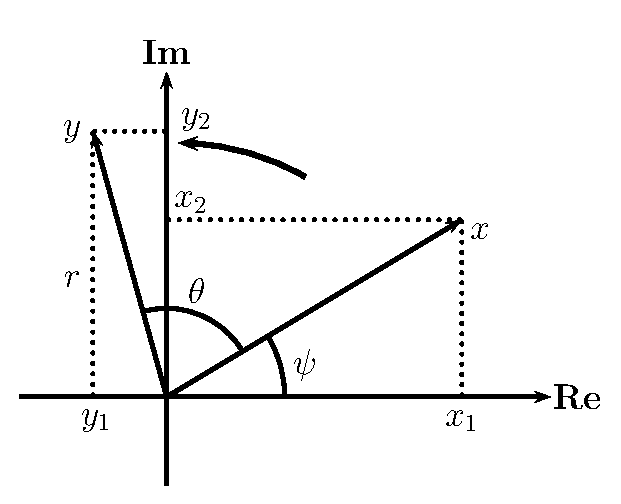
\includegraphics[height=4cm,width=5cm]{FigRotation.eps}
    \end{center}
    \caption{回転写像}
\end{figure}

\section{直交変換}
\subsection{直交行列}
図1はベクトルの長さを変えない写像である.すなわち$\|x\|=\|y\|$.このような長さを保存する写像は
どのような関係を満足しなければならないだろうか? 式(\ref{eq1})より
$$ \|y\|^2 = y^Ty = x^TA^TAx = \|x\|^2 = x^Tx $$
となるためには $x^T(I-A^TA)x=0$ が任意の $x$ に対して成り立たなければならない.したがって
\begin{equation}
    A^TA = I
    \label{eq3}
\end{equation}
が満足されねばならない.式(\ref{eq3})を満足する行列を\textbf{直交行列}(orthogonal matrix)とよぶ.
直交行列の名前は $A$ の列ベクトル $a_1,a_2,\cdots,a_n$ が互いに直交すること,すなわち
\begin{eqnarray}
    a_i^Ta_j =< a_i,a_j >= \delta_{ij} = \left\{\begin{array}{ll}1,& i=j,\\0, & i\neq j \end{array}\right.
    \label{eq4}
\end{eqnarray}
となることからきている.
\par $n \times n$ の直交行列は $n^2$ の要素に式(\ref{eq4})で与えられる $n(n+1)/2$ 個の制約条件が課されるので,その自由度は
$$ n^2-\frac{n(n+1)}{2}=\frac{n(n-1)}{2} $$
である.$n=2$ の場合は式(\ref{eq2})のように1個の自由度である. $n=3$ の場合は3個の自由度が
あり,これは3次元空間におけるベクトルの向きの自由度に対応している.
\subsection{ユニタリ行列}
複素行列$\vect{C}^{n \times m}$の場合は式(\ref{eq3})の代わりに
\begin{equation}
    A^\ast A=I
    \label{eq5}
\end{equation}
を用いる.式(\ref{eq5})を満足する行列を\textbf{ユニタリ行列}(unitary matrix)とよぶ.


\begin{thebibliography}{9}
    \bibitem[1]{kimura}木村英紀,線形代数 数学科学の基礎,東京大学出版会,2003
\end{thebibliography}

\end{document}